\documentclass{mcmthesis}
\mcmsetup{CTeX = true,   % 使用 CTeX 套装时,设置为 true
        tcn = XJ162, problem = A,
        sheet = true, titleinsheet = true, keywordsinsheet = true,
        titlepage = false, abstract = false}
\geometry{left=0.75in,right=0.75in,top=1in,bottom=0.75in}
\numberwithin{figure}{section}
\numberwithin{table}{section}
\numberwithin{equation}{section}
\usepackage{newtxtext}
\usepackage{lipsum}
\usepackage{palatino}
\usepackage{hyperref}
\usepackage{booktabs}
\usepackage{subfigure}
\usepackage{graphicx}
\usepackage{pythonhighlight}
\usepackage{indentfirst}%首段自动缩进
\usepackage{colortbl}
\usepackage{apacite}
\usepackage{natbib}
\usepackage{tablefootnote}
\usepackage{multicol}
%算法四部曲↓
\usepackage{algorithm}
\usepackage{algpseudocode}
\usepackage{amsmath}
\usepackage{algorithmicx}
% \usepackage{threeparttable}

\setlength{\parindent}{2em}
\title{Finless Porpoise PVA based on Vortex, ARIMA, GF and CA}
\setlength{\headheight}{15pt}
\definecolor{darkOrange}{rgb}{0.929,0.49,0.192}
\definecolor{Orange}{rgb}{0.973,0.796,0.678}
\definecolor{lightOrange}{rgb}{0.988,0.894,0.839}
\definecolor{lightBlue}{rgb}{0.867,0.922, 0.969}
\definecolor{lightGreen}{rgb}{0.831,0.929,0.886}
\definecolor{lightYellow}{rgb}{1,0.949,0.8}
\begin{document}
\renewcommand{\algorithmicrequire}{\textbf{Input:}}  % Use Input in the format of Algorithm
\renewcommand{\algorithmicensure}{\textbf{Output:}} % Use Output in the format of Algorithm

\begin{abstract}

In this paper, we predict the population size of the endangered species, Yangtze Finless Porpoise, based on
mathematical models. 
In the first place, we apply \textbf{Vortex model} to calculate the estimated number of 
population in Swan Oxbow and in all ex situ conservation areas. Then, we 
predict the size of population after 20 years by developing \textbf{ARIMA model, 
Gray Forecast model and Cellular Automata model}. With other conditions unchanged, 
the influence of sex ratio over Finless Porpoises in all ex situ protected areas
is assessed by using Vortex model, which is measured by population size and
genetic diversity. In order to estimate whether the functional extinction and
species extinction will occur, we define two kinds of functional extinction, one with 
only one sex left and the other with less than \textbf{200} individuals surviving, whose time 
of occurrence is predicted by Vortex model and Gray Forecast model. 
Finally, we test our model's sensitivity by studying the effects of 
mortality rates over Finless Porpoise population. 
\par
For Problem 1 (a), we use Vortex model to predict the number of Finless Porpoise
population 20 years later in Swan Oxbow, which is \textbf{50}, and in all five ex situ 
conservation areas, which is \textbf{185}. Then we establish ARIMA model, 
Gray Forecast model and Cellular model to predict the number, which is
\textbf{62, 49 and 49}.
\par
For Problem 1 (b), we use Vortex model to calculate the size and the genetic diversity, which
is defined as the normalization of \textbf{GeneDiv} and \textbf{nAlleles} and adjust the male-female 
\textbf{sex ratio from 1:9 to 9:1} to evaluate the impact of sex ratio on Finless Porpoise population. 
It can be discovered that with male proportion growing, 
the number of population shrinks gradually, and the genetic diversity
increases at first, then decreases, approaching its peak when the ratio is \textbf{6:4}.
\par
For Problem 2, we define functional extinction as population with 
less than \textbf{200} individuals or with \textbf{only one sex}. We assess when 
the functional extinction occurs based on Gray Forecast model and 
Vortex model. Based on previous data, Gray Forecast model predicts the
number every five years, and finds that the population will become less than
200 in \textbf{2082}. In other words, it will functionally extinct after \textbf{55 to 60 years}.
Because of the deficiency of ex situ conservation, we change the sex
ratio of Vortex model, the catastrophe probability and mortality rate. It
is predicted by Vortex model that the Finless Porpoises will functionally
extinct after \textbf{55.1 years or 71.3 years}, and will completely extinct
after \textbf{95.5 years}. Based on what has been discussed above, we can 
draw a conclusion that without ex situ conservation, the Finless Porpoises
will functionally extinct after \textbf{55-71.3 years}.
\par
Finally, sensitivity test is carried out based on Vortex model by 
setting additional catastrophes or rising the early mortality rates, and the test
is measured by population size and the extinction. With additional
catastrophes set, the Finless Porpoises will extinct after \textbf{45.3 years}.
With the early mortality rates risen, the extinction will occur after
\textbf{34.8 years}. Thus, both circumstances promotes the probability of
extinction and brings the extinction forward. What's more, it's
found that the increase of early mortality rates influence the development
of the population the most. 

\begin{keywords}
Vortex model, ARIMA time series model, Gray Forecast model, Cellular Automata model, Finless Porpoises in Yangtze River, Population viability analysis.
\end{keywords}
\end{abstract}
\maketitle

\tableofcontents
  \thispagestyle{empty}
  \newpage
  \setcounter{page}{1}
%%
%%Generate the Memorandum, if it's needed.
%\memoto{\LaTeX{}studio}
%\memofrom{Liam Huang}
%\memosubject{Happy \TeX{}ing!}
%\memodate{\today}
%%\logo{\LARGE I'm pretending to be a LOGO!}
%\begin{memo}[Memorandum]
%  \lipsum[1-3]
%\end{memo}

\section{Introduction}

\subsection{Problem Restatement}

Finless Porpoise is the only freshwater mammal in the Yangtze River at present, 
which is distributed in the middle and lower reaches of the Yangtze 
River, Dongting Lake and Poyang Lake, and its population has 
decreased dramatically in the past 20 years. According to the statistics, 
the number of Finless Porpoises in the Yangtze River was more than 2,700 in 1991. 
However, in the year of 2006, there were fewer than 1,800 Finless Porpoises surviving in the area. 
In 2011, there were probably just over 1,000 of them, and in 2018 there were about 1,012. 
\par
In fact, since the 1980s, the ecologists along with the government
had explored and developed three conservation strategies: 
in situ conservation, ex situ conservation and artificial breeding.
Among them, ex situ protection, that is, selecting some waters with 
similar ecological environment to the Yangtze River to establish 
ex situ protection, is the most direct and effective measure
to protect the Yangtze Finless Porpoise. 
\par
China has set up five ex-situ protected sites until now, in which 
more than 150 Yangtze Finless Porpoises are conserved. On September 18, 2021, CCTV reported that 
the population of the Yangtze Finless Porpoise is growing steadily. 
The population decline of the Yangtze Finless Porpoise has been 
curbed, but its critically endangered status remains unchanged.
\par
Based on what has been discussed above, please address the following problems:
\begin{enumerate}
  \item [1] \begin{enumerate}
    \item Establish a mathematical model to predict the population number of Finless Porpoises in five ex situ protected areas after 20 years.
    \item Explain how the sex ratio of 150 Finless Porpoises in ex situ protected areas affects the population development of Finless Porpoises.
  \end{enumerate}
  \item [2] Will the Yangtze Finless Porpoise become functionally extinct without ex situ conservation strategies?
  \item [3] Based on your analysis, please submit no more than 2 pages of recommendations for the protection of Finless Porpoises to the relevant authorities.
\end{enumerate}

\subsection{Overview of Our Work}
We develop 4 kinds of models to fully assess the trend in terms of 
annual change of finless population size in Swan Oxbow, which are 
furthermore applied on all five ex-situ protected areas to predict 
the change of population. 
\par
Besides, Vortex model, as the most comprehensive
and authoritative model widely used in studying small-size populations of
creatures, is the core for analyzing the viability of finless 
porpoise population from different perspectives, especially when 
the discussion of sex ratio is involved.
\par
For more clear and general information of our work, please see 
Figure \ref{Frame}.
\newpage
\begin{figure}[htbp]
  \centering
  \includegraphics[width =13cm]{codes/框架图.pdf}
  \caption{Frame Diagram of our work}\label{Frame}
\end{figure}




\section{Assumptions and Justifications}
These are necessary assumptions for simplifying the model.
\begin{enumerate}
  \item [1.] The initial carrying capacity per unit area of each ex-situ conservation layout is constant;\label{assumption1}
  \item [2.] The carrying capacity of Finless Porpoise in Yangtze River is 3000, and there is no large-scale migration of Finless Porpoises in adjacent 
  monitored river segments within a certain period of time\citep*{Xiongyuanhui};
  \item [3.] Assume that carrying capacities for Finless Porpoises decline 10\% every year;
  \item [4.] Under natural conditions, it is assumed that there 
  are two natural disasters affecting the population of finless 
  porpoise, namely, the blasting operation in the Yangtze River 
  channel and the capsizing accident of the ship carrying 
  pesticides in the Yangtze River, which happen once every 
  10 years. According to the field observation, 
  the reproductive rate and survival rate of the population 
  of Finless Porpoise decreased to 95 percent after the disaster \citep*{Zhangxianfeng};
  \item [5.] Under ex situ conservation conditions, it is assumed 
  that there are following advantages in the reserve environment, 
  and the mortality rate of each age of Finless Porpoise population is 
  greatly reduced, and only one disaster exists;
  \item [6.] Suppose the mortality rates of male and female Finless Porpoises are significantly different;
  \item [7.] Assume that no artificial harvest and supplement;
  \item [8.] Assume that the reproductive system of the Finless Porpoise is polygynous;
  \item [9.] Assume all Finless Porpoises in Yangtze River belongs to the same population.
\end{enumerate}


\section{Notations}

\renewcommand\arraystretch{1.5}

\begin{table}[htpb!]
  \centering
  \caption{Notation Descriptions\citep{Vortex}} \label{Vortex_out}
  \begin{tabular}{m{2.5cm}<{\centering}|m{12.5cm}<{\centering}}
  \toprule[1.5pt]
  \textbf{Symbol} & \textbf{Definition} \\ \hline
  $ r $ & Innate rate of increase \\
  Stoch r & The mean population growth rate experienced in the simulations, averaged 
  across all years in which the population was extant. \\
  %内廪增长率:给定的物理和生物的条件下,具有稳定的年龄组配的种群的最大瞬时增长率
  N-extant  & Average extant population size\\ 
  N-all  & Average population size \\
  PE  & Probability of Extinction \\
  GeneDiv  &  Genetic Diversity \\
  TE & Time of Extinction(year) \\
  medianTE & If at least 50\% of the iterations went extinct, 
  the median time to extinction \\
  SD & Standard Deviation \\
  nAlleles & The mean number of alleles remaining within extant populations 
  (from an original number equal to twice the number of founder individuals)\\
  $ K $ & Carrying capacity \\ 
  $ N_t $ & Size of Finless Porpoise population in the year of $ 1991 + t $ \\ 
  \bottomrule[1.5pt]
  \end{tabular}
  \end{table}



\section{Introduction and Results of Models on Problem 1(a)}


Considering tremendous cost on massive Finless Porpoise population 
census, merely six years of data was collected in Swan Oxbow of the Yangtse River
during the three decades since 1992. \citep*{Liuzhigang}
Thus, we've applied \textbf{Lagrange interpolation} to obtain other years' data
in Swan Oxbow.

 

\subsection{Relation between Population Size and Time based on Lagrange Interpolation}
Given $ n $ distinct real values $ x_1, x_2, \cdots , x_n $and $ n $
real values $ y_1, y_2,\cdots, y_n $ (not necessarily distinct), there
is a unique polynomial $ P $ with real coefficients satisfying 
$ P(x_i)= y_i $ for $ i \in \{1,2,\cdots,n\} $, such that deg($ P $ )<n.
\par
The polynomial $ P(x) $ is defined as follows:   
$$
  P(x) = \sum \limits _{k = 1}^ny_kp_k(x),\quad
  p_k(x) = \frac{(x-x_1)\cdots (x-x_{k-1})(x-x_{k+1})\cdots (x-x_n)}{
    (x_k-x_1)\cdots (x_k-x_{k-1})(x_k-x_{k+1})\cdots (x_k-x_n)
  }
$$

After substituted the number in 1992, 2002, 2005, 2007, 2015 and 2021,
the figure of the polynomial is as follows:
\begin{figure}[htbp!]
  \centering
  \includegraphics[width = 8cm]{codes/Lagrange.eps}
  \caption{Langrange Interpolation Conservation}
\end{figure}

\par
According to Lagrange interpolation and the definition of $ N_t $ :
$$
  N_t = P(t) \quad t = 1,\cdots ,30
$$ 
and the exact numbers are listed below:
\begin{table}[htpb!]
  \centering
  \caption{Estimated size of population on year basis from 1992 to 2022} \label{Lagrange table}
  \begin{tabular}{m{2cm}<{\centering}|m{2cm}<{\centering}|m{2cm}<{\centering}|m{2cm}<{\centering}|m{2cm}<{\centering}|m{2cm}<{\centering}}
  \rowcolor{lightBlue}  \textbf{Year}&\textbf{Number}&\textbf{Year}&\textbf{Number}&\textbf{Year}&\textbf{Number}\\ \hline
  \rowcolor{White}  1992 & 5       & 2002 & 20      & 2012 & 45.7364 \\
  \rowcolor{lightBlue}  1993 & 10.4864 & 2003 & 21.2919 & 2013 & 49.2555 \\
  \rowcolor{White}  1994 & 13.9987 & 2004 & 22.9647 & 2014 & 52.9737 \\
  \rowcolor{lightBlue}  1995 & 16.0839 & 2005 & 25      & 2015 & 57      \\
  \rowcolor{White}  1996 & 17.2014 & 2006 & 27.3612 & 2016 & 61.4941 \\
  \rowcolor{lightBlue}  1997 & 17.7296 & 2007 & 30      & 2017 & 66.6734 \\
  \rowcolor{White}  1998 & 17.9732 & 2008 & 32.8636 & 2018 & 72.82   \\
  \rowcolor{lightBlue}  1999 & 18.1701 & 2009 & 35.9015 & 2019 & 80.2876 \\
  \rowcolor{White}  2000 & 18.4981 & 2010 & 39.0724 & 2020 & 89.5084 \\
  \rowcolor{lightBlue}  2001 & 19.0819 & 2011 & 42.3514 & 2021 & 101     \\
  \end{tabular}
\end{table}
\newpage
\subsection{Model I: Vortex model based Finless Porpoise analysis}
Primary functional principles of Vortex model are shown in the form of
pseudocode Algorithm \ref{Alg:vortex}. 

\begin{algorithm}[htbp]
  \caption{Vortex model based Finless Porpoise Population Size Prediction Algorithm} % 名称
  \label{Alg:vortex}
  \begin{algorithmic}[1]
    \Require
      features of Finless Porpoises described in table \ref{Vortex_in}
      \For{scenario $ \gets 1$ to $ m $}
      \If{NumberOfPopulations $ \geq 1 $ } 
      \State READ POPULATION and MIGRATION
      \For{each population, pSource $ \gets 1 $ to $ n $  }
      \State $ BreedEV[P] = \sqrt{BreedEV[P]^2-BreedEV[P]\times EVConcordance} $
      \State Calculate the parameters $ \gets $ LOCAL\_EV, CATASTROPHES, MIGRATE, BREED, MORTALITY(p)
      \EndFor
      \For{each Year $ \gets 1 $ to $ l $  }
      \State $SE = \sqrt{PE \times (1-PE)} $
      \If{population extincted}\State $ Year Recolonized[P] = Current Year $ 
      \Else \State $ TimeToRecolonization[p] = CurrentYear - YearExtinct[p]$ 
      \EndIf 
      \If{not extinct $\&\&  PopulationSize[p], N > Carrying Capacity[p] $ }
      \For{each indiividual}
      \If{$ RAND() > \frac{K}{N} $}
      \State Extinct
      \Else \If{$ N>K $} 
      \State $ YearExtinct[p] = CurrentYear $
      \EndIf
      \If{others} 
      \State $ TimeToReextinction[p] = CurrrentYear- Recolonization[p] $ 
      \EndIf
      \EndIf
      \EndFor
      \EndIf
      \EndFor
      \EndIf
      \EndFor
      \Ensure
      The Number of iterated population in each year
  \end{algorithmic}
\end{algorithm}

By inputting pre-set parameters (see Table \ref{Vortex_in}), 
carrying capacity $ K = 101 $ and present population size $ N_0 = 82 $
(both numbers come from news in People's Daily, and 19 Finless Porpoises were
moved from Swan Oxbow to other ex situ conservation areas in 2021) in Swan Oxbow, we learn from
Vortex model that the population size reaches its peak of \textbf{88.84}, and 
than declines and stabilizes at about \textbf{50}.
\par
According to our assumptions \ref{assumption1}, we assume the carrying capacity for five ex-situ protected areas 
$ K = 369 $. Vortex shows that the number roars to \textbf{241.26} in the forth 
year, and then settles around \textbf{185}. 

\subsection{Model II: Auto Regressive Integrated Moving Average(ARIMA) model}
We apply ARIMA model in order to predict the size of Finless Porpoise population in five ex-situ 
conservation areas after 20 years, whose \textbf{algorithm block diagram} 
is shown as Figure \ref{ARIMA_ALGO}.
\par
Under regular circumstances, the time series we obtain in the real world
  has tendency, seasonality and non-stationarity. Thus, it's vital for 
  us to transfer the non-stationary time series to stationary time series
\par
\begin{figure}[ht]
\begin{minipage}[htbp]{0.35\linewidth}
  and make an assumption that the time series is an Auto 
  Regressive Moving Average(ARMA) series to predict the 
  future data. ARMA series is defined as follows.
  \begin{align*}
    &X_t-\phi_1X_{t-1}-\cdots -\phi_pX_{t-p} \\
    &= \epsilon_t - \theta_1\epsilon_{t-1}-\cdots-\theta_q\epsilon_{t-q}
  \end{align*}
 
$ \epsilon_1 $ is a stationary white noise whose average is zero and
deviation is $ \sigma_\epsilon^2 $;$ X_t $is an ARMA series with $ p $ and $ q $
degree, recorded briefly as $ \mathbf{ARMA}(p,q) $ series.
Akaike Information Criterion(AIC) is one of the most commonly used
criterion to determine the degree of $ \mathbf{ARMA}(p,q) $: choose 
$ p,q $ such that 
\begin{equation}\label{AIC}
  \begin{aligned}
    \min \mathbf{AIC} &= n\ln \hat{\sigma_\epsilon^2} \\
    &+ 2(p+q+1)
  \end{aligned}
\end{equation}
$ n $ is the capacity of sample;$ \hat{\sigma_\epsilon^2} $ is the
estimation of $ \sigma_\epsilon^2 $ relating to $ p $ and $ q $.
Suppose $ p = \hat{p}, q = \hat{q} $, such that equation(\ref{AIC}) reaches the minimum,
than we deem the series is $ \mathbf{ARMA}(\hat{p},\hat{q}) $. 
\end{minipage}
\hfill
\begin{minipage}[htbp]{0.55\linewidth}
  \begin{flushleft}
    \includegraphics[width =11cm]{codes/ARIMA_裁剪页面.pdf}
   \caption{Algorithm Block of ARIMA}\label{ARIMA_ALGO}
  \end{flushleft}
\end{minipage}
\end{figure}



\par
Suppose $ \mathbf{ARMA}(p,q) $ series has an unknown average parameter $ \mu $,
the model becomes
$$
  \phi(B)(X_y-\mu) = \theta(B)\epsilon_t,
$$   
meanwhile, the number of unknown parameters is $ k = p+q+2 $, the AIC is:
choose $ p,q $ such that
\begin{equation}\label{AIC_unknown}
  \min \mathbf{AIC} = n\ln\hat{\sigma_\epsilon^2}+2(p+q+2).
\end{equation}  
In fact, equations (\ref{AIC}) and (\ref{AIC_unknown}) have the same minimum point $ \hat{p},\hat{q} $.
After that, we usually choose $ p = 1, q = 1 $ to make parameter estimation 
over ARMA model.
\par
It's demonstrated that the differential operation can stabilize 
certain class of non-stationary series. And It's emphasized that 
stationary test must be conducted previously. Stationary test can 
be applied by calculating sample autocorrelation function and 
sample coefficient of partial function. 
\par
If the functions are truncated or trending to 0 (meaning being controlled
by negative index), than the series belongs to ARMA model.
\par
If at least one of the functions above is not truncated or trending to 0, than
it's not stationary.
\par
Suppose the series is non-stationary, which can be transformed to 
a stationary series by $ d $ -degree differential operation, denoted
as $ \mathbf{ARIMA}(p,q,d) $ series,than differentiate the sample by
$ d $ -degree:
$$
  W_t = \nabla^dX_t,\quad t = d+1,\dots , n
$$ 
After that, apply stationary test on $ W_t $ and repeat steps above 
until it becomes a stationary series, Than $ W_t $(which is denoted
as $ X_t $ ) complies ARMA model. 
\par
The figures below describe the result of ARIMA model on the 
time series of the size of Finless Porpoise $ N_t, \quad t = 1\cdots 30 $,
in which the Figure(\ref{ARIMA Sequence}) clearly shows that the number
will decline and settle around \textbf{62} in the future 20 years. 



\begin{figure}[htbp]
  \centering

  \subfigure[Sample Autocorrelation Function and Sample Partial Autocorrelation Function]{
  \centering
  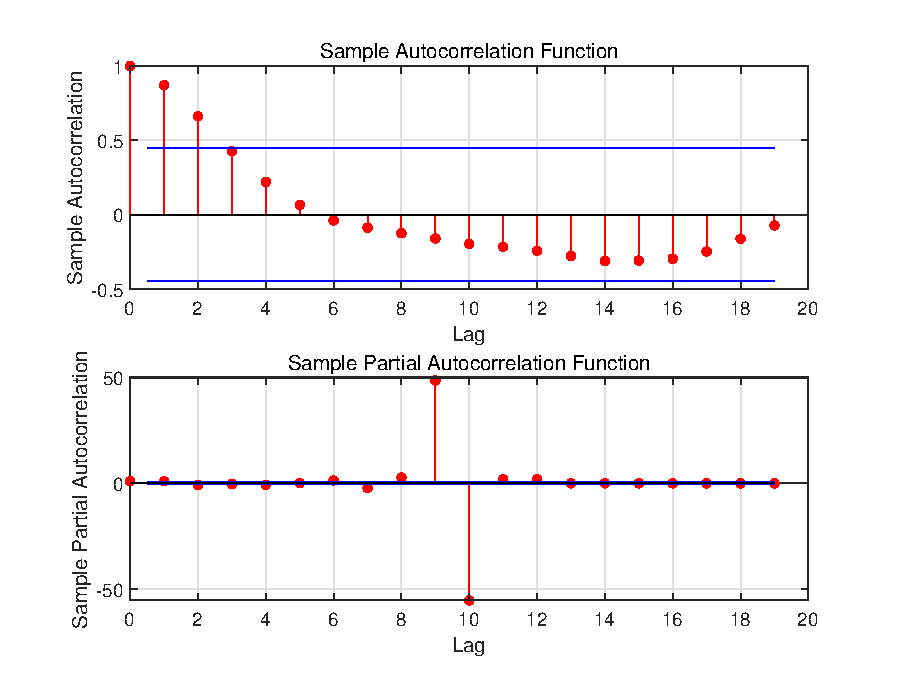
\includegraphics[width = 0.3\textwidth]{codes/1.eps}
  }
\quad
  \subfigure[Sample Autocorrelation Function and Sample Partial Autocorrelation Function]{
  \centering
  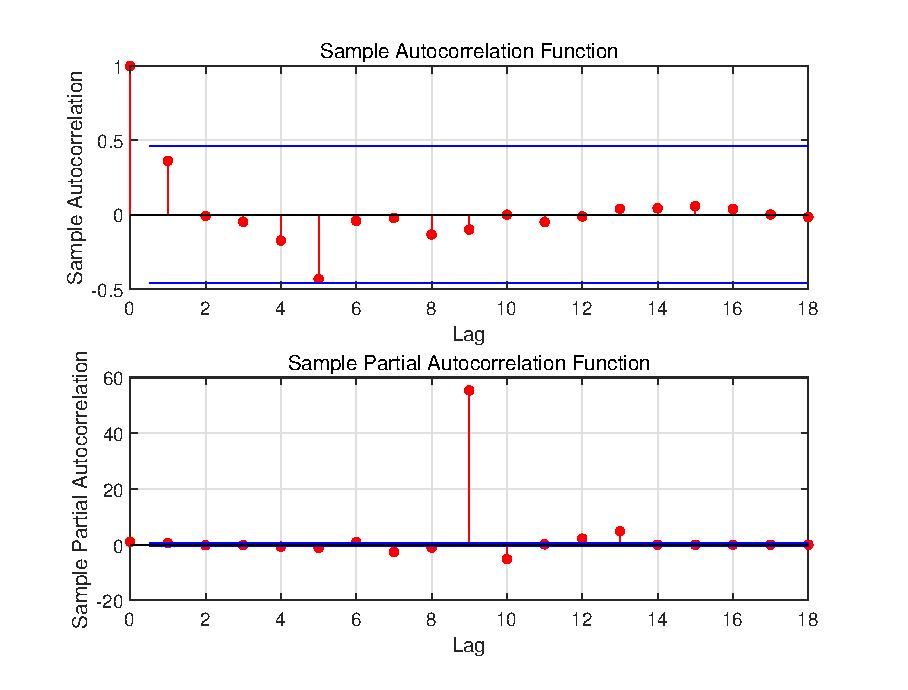
\includegraphics[width = 0.3\textwidth]{codes/3.eps}
  }
\par
  \subfigure[ARIMA Sequence Prediction of Conservation]{
  \centering
  \includegraphics[width = 0.3\textwidth]{codes/2.eps}\label{ARIMA Sequence}
  }
\quad
\subfigure[Standardaized Residuals and QQ figure]{
  \centering
  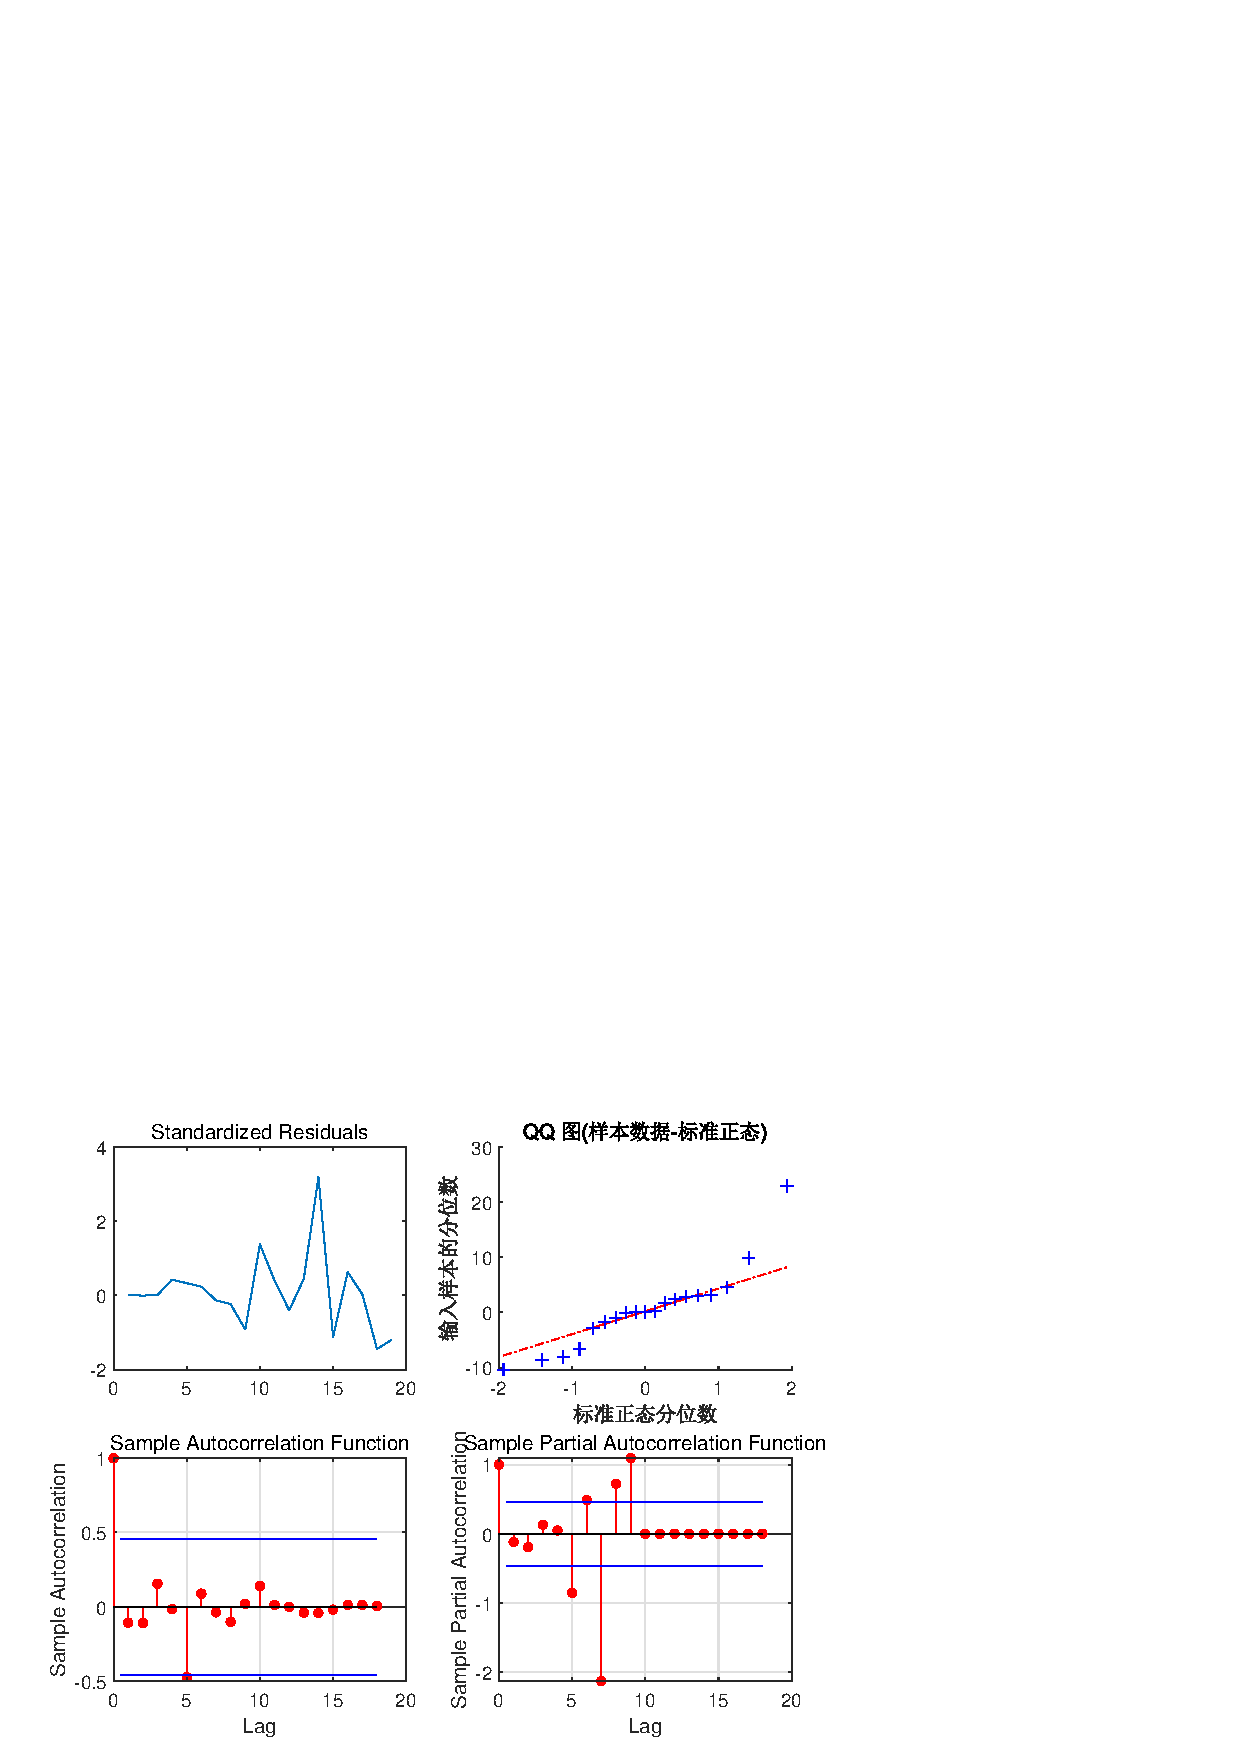
\includegraphics[width =0.3\textwidth]{codes/4.pdf}
}
\caption{Results of ARIMA model}
\end{figure}

\newpage











\subsection{Model III: Cellular Automata based Population Size Prediction}

Cellular automata (CA) is a kind of grid dynamics model with discrete time, 
space and state, and local spatial interaction and temporal causality, which 
has the ability to simulate the space-time evolution process of complex system.
\par
Unlike general dynamical models, cellular automata are not determined by strictly 
defined physical equations or functions, but are composed of rules constructed by 
a series of models. Any model that satisfies these rules can be regarded as a cellular 
automata model. Therefore, cellular automata is a general term for a class of models, 
or a method framework. Its characteristic is that time, space and state are discrete, 
each variable only takes a finite number of states, and its state change rules are local 
in time and space.
\par
The block diagram of a typical cellular automata is shown in Figure \ref{CA_Fig}, 
and the simulation result is shown in Figure \ref{CA_reslut}, in which
we learn that the predicted number of population in Swan Oxbow is \textbf{49}.


\begin{figure}[htbp]
  \centering
  \includegraphics[width = 14cm]{codes/元胞自动机流程图.pdf}
  \caption{Block Diagram of typical Cellular Automata}\label{CA_Fig}
\end{figure}





\begin{figure}[htbp]
  \centering
  \subfigure[Living Environment Index and Population]{
    \centering
    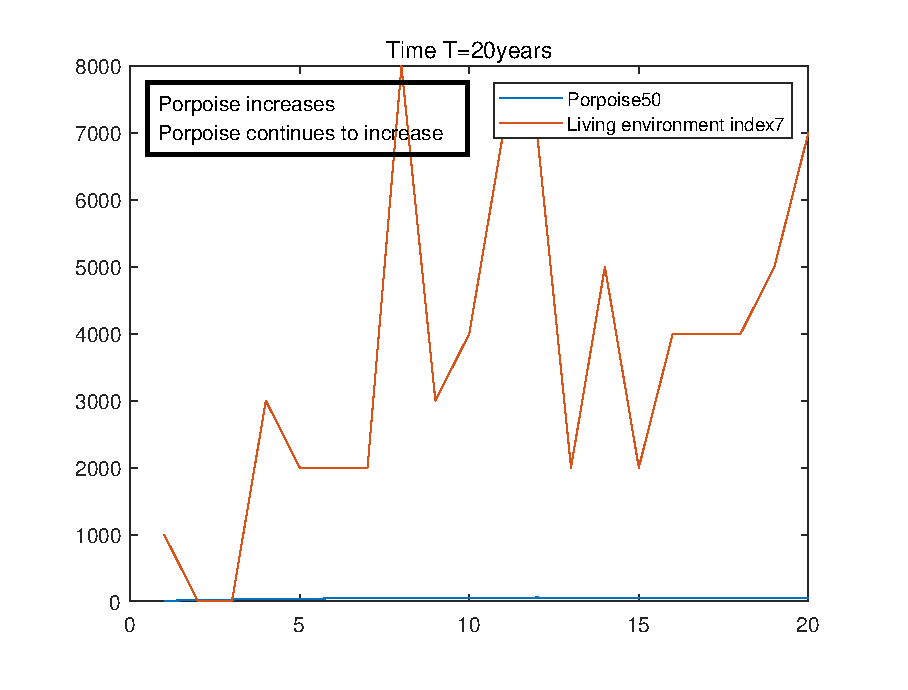
\includegraphics[width = .45\textwidth]{codes/20(1).eps}
    \quad
    }
  \subfigure[Cell Distribution]{
    \centering
    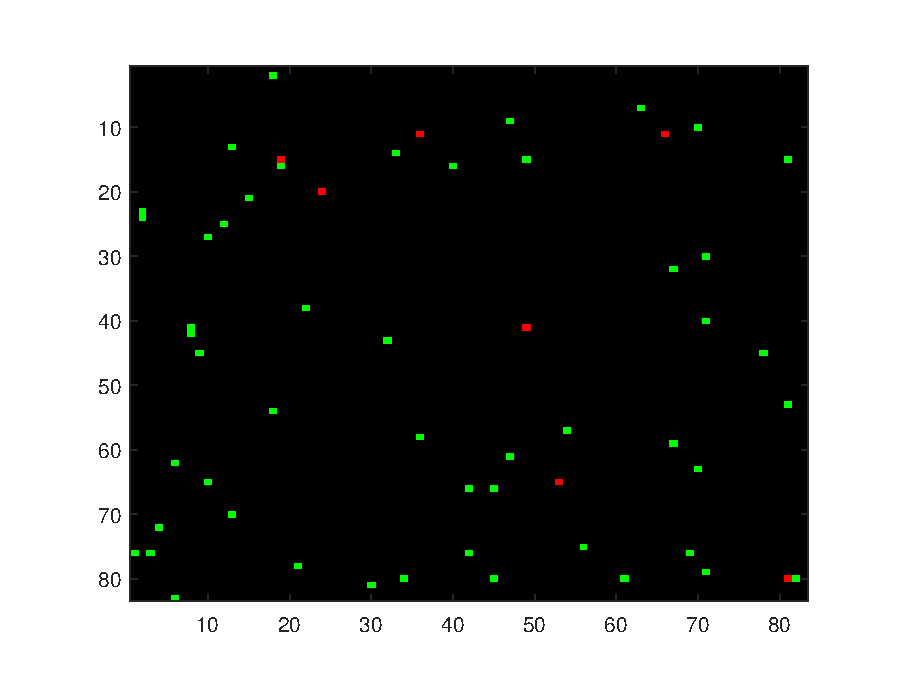
\includegraphics[width=.45\textwidth]{codes/20(2).eps}
  }
  \caption{Results of CA Simulating Population in Swan Oxbow}\label{CA_reslut}
\end{figure}










\subsection{Model IV: Gray Forecast model}

The very heart of Gray Forecast is Gray model, which is used to model and 
forecast the approximate exponential law after summing up the 
original data. It is suitable for the prediction scenario with 
less data. While \textbf{Vehulst} model is primarily used to
describe procedures with saturation state, that is S-shape procedure,
which can be applied in the sphere of biological growth and reproductive prediction.
The fundamental is as follows.
\par
Suppose the sample is $ x^{(0)} = \{x^{(0)}(1), x^{(0)}(2) \cdots
x^{(0)}(n)\} $, and it is accumulated once to generate a 
(1-AGO) sequence, which is:
$$
  x^{(1)} = (x^{(1)}(1),x^{(1)}(2),\cdots, x^{(1)}(n))
$$ 
$ z^{(1)} $ is the mean-generating sequence of $ X^{(1)} $, which is:
$$
z^{(1)} = (z^{(1)}(2),z^{(1)}(3),\cdots,z^{(1)}(n)).
$$ 
Then, we call the following equations Gray Verhulst model with parameters a and b:
$$
  x^{(0)} + az^{(1)} = b(x^{(1)})^2
$$ 
, and we call the following equations the winterization equations of
of Gray Verhulst model with t denoting time:
$$
  \frac{\mathbf{d}x^{(1)}}{\mathbf{d}t} + ax^{(1)} = b(x^{(1)})^2
$$ 
\par
\textbf{Theorem 1}. Suppose the Gray Verhulst model is depicted as above, if
$ \bm{u} = [a,b]^T $  is the parameter vector,and 
$$
  \bm{B} = 
  \begin{bmatrix}
    -z^{(1)}(2) & (z^{(1)}(2))^2\\
    -z^{(1)}(3) & (z^{(1)}(3))^2\\
    \vdots & \vdots\\
    -z^{(1)}(n) & (z^{(1)}(n))^2
  \end{bmatrix},
  \bm{Y} = \left(
  \begin{array}{c}
    x^{(0)}(2)\\
    x^{(0)}(3)\\
    \vdots\\
    x^{(0)}(n)
  \end{array}\right),
$$
then the least square estimation of parameter $ \bm{u} $ satisfies
$$
  \hat{\bm{u}} = [\hat{a},\hat{b}]^T = (\bm{B}^T\bm{B})^{-1}\bm{B}^T\bm{Y}
$$ 

\textbf{Theorem 2}
Suppose Gray Verhulst model is defined as above, then solution to the winterization
equations is 
$$
  x^{(1)}(t) = \frac{\hat{a}x^{(0)}(1)}{\hat{b}x^{(0)}(1)+[\hat{a}-\hat{b}x^{(0)}(1)]e^{\hat{a}t}},
$$ 
and the time response sequence of Gray Verhulst model is
$$
  \hat{x}^{(1)}(k+1) = \frac{\hat{a}x^{(0)}(1)}{\hat{b}x^{(0)}(1)+[\hat{a}-\hat{b}x^{(0)}(1)]e^{\hat{a}t}},
$$ 
and the reductive formula is 
$$
  \hat{x}^{(0)}(k+1) = \hat{x}^{(1)}(k+1) - \hat{x}^{(1)}(k)
$$ 

\par
After developing basic rules of Gray Forecast model, we deploy it on
the analysis of the Finless Porpoise size in future 20 years. 
\par
Suppose the number series of Finless Porpoise is
$$
N^{(0)} = (N^{(0)}(1),N^{(0)}(2),\cdots, N^{(0)}(n)).
$$ 
Then we accumulate it and generate Verhulst series:
$$
N^{(1)} = (N^{(1)}(1),N^{(1)}(2),\cdots, N^{(1)}(n)),
$$ 
Thus, we can get Verhulst differential equations:
$$
\frac{\mathbf{d}N^{(1)}}{\mathbf{d}t} + aN^{(1)} = u
$$ 
, in which $ a $ and $ u $ is defined as above. Further more, 
we could solve the following equations to get the answer:
$$
\bm{B} = 
\begin{bmatrix}
  -\frac{1}{1}[N^{(1)}(1)+N^{(1)}(2)]\\
  -\frac{1}{2}[N^{(1)}(1)+N^{(1)}(3)]\\
  \vdots \\
  -\frac{1}{2}[N^{(1)}(n-1)+N^{(1)}(n)]
\end{bmatrix},
\bm{Y_n} = \left(
\begin{array}{c}
  N^{(0)}(2)\\
  N^{(0)}(3)\\
  \vdots\\
  N^{(0)}(n)
\end{array}\right),
$$  

$$
  \hat{N^{(1)}(k+1)} = [N^{(0)}(T)-\frac{\hat{u}}{\hat{a}}]e^{-\hat{a}k}+\frac{\hat{u}}{\hat{a}}
  \quad k = 0,1,\cdots, n
$$ 

After iterating based on Table \ref{Lagrange table}, Gray Forecast model
comes with a prediction of \textbf{49.308} after 20 years in Swan Oxbow.


\section{Solution to Problem 1(b) based on Vortex model}
Considering the abundant parameter settings in Vortex software among which sex ratio 
is easy to edit and is of great significance, we decide to further apply Vortex model
in order to address the problem 1(b) concerning the effects of sex ratio in five ex-situ
conservation zones.
\par
In order to more comprehensively demonstrate the impact of sex ratio, 
we compare the surviving condition 20 years later with male-female ratio ranging 
from $ 1:9 $ to $ 9:1 $. We regard the number of population as one important
factor, and the Genetic Diversity, which is defined as \textbf{the normalization of}
$ \bm{GeneDiv + nAlleles} $, as the other. The result is shown in Figure \ref{Sex-Pop}.  
\begin{figure}[htbp]
  \centering
  \includegraphics*[width = 12cm]{codes/影响.pdf}
  \caption{Influence of Sex Ratio over Population Size}\label{Sex-Pop}
\end{figure}

From the Figure \ref{Sex-Pop} could draw a very reasonable conclusion that
the larger the male-female ratio is, the more damage it will cause to the
survival of whole population, which corresponds with Finless Porpoise's 
polygyny. 

\section{Vortex model and Gray Forecast model based
Population Prediction without Ex-Situ Conservation}

The known \textbf{existing wild Finless Porpoise population is 1012} \citep*{Wubin}. 
According to previous researches, female Finless Porpoises are more
vulnerable than the male ones in their early ages, so the ratio of 
male Finless Porpoises to female ones which are 0-6 years old is $ 3.7:1 $
\citep*{ZhouZhao},
and the ratio of those older than 6 is $ 2:1 $. For simplicity, 
we perceive that \textbf{the ratio of male Finless Porpoises to female ones
in all ages} is $ \bm{2.85:1} $, which is the median of the above two ratios.
What's more, we assume that \textbf{the carrying capacity} $ K $  of Finless Porpoises
in the whole Yangtze River is \textbf{3000}.
\par
In order to thoroughly discuss the risk of Finless Porpoise extinction,
we define two types of \textbf{functional extinction} and one type
of \textbf{species extinction}. 
\par
The first type of functional extinction 
(\textbf{Functional Extinction I}) is that there only exists one 
sex, which means this population is no longer able to reproduce and bond 
to be extinct in the future.
\par
The second type of functional extinction
(\textbf{Functional Extinction II}) is that the number of 
remaining individuals in the population is unable to prevent inbreeding
depression which will cause the fading and extinction of the population.
We define the number of population that reaches the second functional 
extinction is \textbf{200}.
\par
The \textbf{Species Extinction} is defined as no living individual of this population
found in this area. 

\subsection{Result of Vortex model}\label{Prob_2_VortexSection}
The result of Vortex model simulation based on previous conditions 
is shown as Table \ref{Vortex_result_2}, in which the meaning of 
these parameters is shown in Table \ref{Vortex_out}.

\begin{table}[htbp]\label{Vortex_result_2}
  \centering
  \begin{tabular}{
  >{\columncolor[HTML]{ddebf7}}c |ccc}
  \textbf{Scenario} &
    \cellcolor[HTML]{ddebf7}\textbf{Species Extinction} &
    \cellcolor[HTML]{ddebf7}\textbf{Functional Extinction I} &
    \cellcolor[HTML]{ddebf7}\textbf{Functional Extinction II} \\ \hline
  \textbf{nRuns}     & 30      & 30      & 30      \\
  \textbf{stoch-r}   & -0.0239 & -0.0165 & -0.0120 \\
  \textbf{SD(r)}     & 0.1399  & 0.1340  & 0.1359  \\
  \textbf{PE}        & 0.0667  & 0.1000  & 0.4667  \\
  \textbf{N-extant}  & 256.00  & 340.00  & 427.25  \\
  \textbf{SD(N-ext)} & 259.57  & 257.31  & 214.72  \\
  \textbf{N-all}     & 238.93  & 306.03  & 268.37  \\
  \textbf{SD(N-all)} & 258.75  & 264.76  & 236.37  \\
  \textbf{GeneDiv}   & 0.8852  & 0.9300  & 0.9621  \\
  \textbf{SD(GD)}    & 0.1257  & 0.0321  & 0.0132  \\
  \textbf{nAlleles}  & 31.71   & 35.59   & 51.56   \\
  \textbf{SD(nA)}    & 20.83   & 19.06   & 16.43   \\
  \textbf{medianTE}  & 0       & 0       & 80      \\
  \textbf{meanTE}    & 95.5    & 71.3    & 55.1   
  \end{tabular}
\end{table}

In a nut shell, from the \textbf{meanTE} value in Table \ref{Vortex_result_2}
we can draw a reasonable conclusion that without ex-situ conservation actions, 
the Finless Porpoises in Yangtze River will suffer \textbf{Functional Extinction II after 
55.1 years, Functional Extinction II after 71.3 years and Species Extinction
after 95.5 years.}

What's shown in Figure \ref{ExtinctionPic} describes the variation trends in these scenarios.




\subsection{Result of Gray Forecast model}
Given the fact that the Gray Forecast model is unable to predict the date of
Functional Extinction I, we deploy the model to measure Functional Extinction II. 



The Figure \ref{Gray_Pridct} has explicitly shown that it will take
the Finless Porpoise population 55 to 60 years to reach Functional
Extinction II, which is unbelievably similar to the conclusion of
Vortex model from section \ref{Prob_2_VortexSection}.

\begin{table}[htpb!]
  \centering
  \caption{Values inputted into Vortex\citep{Zhangxianfeng}} \label{Vortex_in}
  \begin{tabular}{m{12.5cm}<{\centering}|m{2.5cm}<{\centering}}
    \toprule[1.5pt]
    Times simulated & 1000times \\
    Years simulated & 100a \\
    Reporting interval &  10a\\
    Populations simulated  & 1\\ 
    Inbreeding depression (Y/N)  & Y \\
    Heterosis or Lethal  & H \\
    Lethal equivalents  &  3.14 \\
    EV correlation between reproduction and survival & 0.5 \\
    EV correlation among populations & 0.5 \\
    %此处这两个EV correlation可以选择性扩展解释(Vortex manual)
    Types of catastrophe & 2 \\ 
    Monogamous, Polygynous or Hermaphroditic & P \\
    Female breeding age & 4a\\
    Male breeding age & 5a\\
    Maximum breeding age & 15a\\
    Maximum litter size & 1\\
    $ P(0) $ (the percent 
    of adult females that breed at low densities when there is no Allee effect)  & 70\% \\
    $ P(K) $ (the percent that 
    breed when the population is at carrying capacity) & 25\% \\
    B & 2\\
    A & 2\\
    Percent litter size 1& 100\%\\
    Moralities in different ages & see Table \\%%%
    Catastrophes and influence & see Table \\%%%%%%%%
    Percent males in breeding pool & 70\% \\
    Start at stable age distribution (Y/N)? & Y \\
    Trend in K (Y/N) ? & Y \\
    Years of trend & 5a\\
  \end{tabular}
\end{table}

\begin{table}[htpb]
  \centering
  \begin{tabular}{m{12.5cm}<{\centering}|m{2.5cm}<{\centering}}
    Years of trend & 5a\\
    Percent age in K & -10\%\\
    Harvest (Y/N)? & N\\
    Supplement (Y/N)? &N\\
    Sex ratio (proportion males) at birth\tablefootnote{Modifiable when discussing different scenarios.} & 0.5\\
    Density dependent breeding\tablefootnote{$ P(N) $  is the percent of females the breed when the population size is $ N $, 
    which can be difined as $ P(N) = P(0) - [P(0)-P(K)(\frac{N}{K})^B]\frac{N}{N+A} $ } (Y/N)? & Y\\


    \bottomrule[1.5pt]
  \end{tabular}
\end{table}

\begin{figure}[htbp]\label{Gray_Pridct}
  \centering
  \includegraphics[width = 9cm]{codes/gray.eps}
  \caption{Predicted Population Size based on Gray Forecast}
\end{figure}


\section{Sensitivity Test}
In order to implement sensitivity test, we make two basic assumptions
and study whether the result coincides with our assumptions.
\par
First assumption is that under the influence of human activities, 
the environment of the Yangtze River will deteriorate further 
in the future, and the factors threatening the survival of the 
Finless Porpoise will develop further, which will lead to the 
increase of the mortality rate of the young population of the 
Finless Porpoise. More precisely, 30\% of Finless Porpoises in their
0 to 2 years old would die due to Environmental Variations. 
\par

The second assumption is that as the environment of the Yangtze river deteriorates, 
there is a possibility that the habitat of Finless Porpoises will 
shrink further and that factors that were previously unlikely 
to be a disaster, such as an epidemic outbreak, will become a 
disaster. Suppose that the probability of an epidemic is 10\%, 
that 10\% of individuals will die from the disease, and that 
10\% of individuals will be severely affected in reproduction.
\par
Under assumptions described above, we apply Vortex model to see whether the 
extinction probability of the Finless Porpoise will be greatly increased.

\begin{figure}[htbp]
  \centering
  \subfigure[Number of Finless Porpoise population in higher early death rate]{
    \centering
  \includegraphics[width = 7cm]{codes/mortality.png}}
  \quad
  \subfigure[Number of Finless Porpoise population in epidemic]{
    \centering
  \includegraphics[width= 7cm]{codes/3种灾害.png}}
  \caption{Sensitivity Test}\label{Sensitivity}
\end{figure}

From Figure \ref{Sensitivity} and the result of Vortex model, we can
see clearly that for the first assumption, which consists of 30\%
early death, it will take the Finless Porpoises \textbf{34.8} years to
functionally extinct (type II), which is significantly shorter than the 
natural situation of 55.1 years; for the second scenario, the functional
extinction comes after \textbf{45.3} years, which is also less than the 
natural situation.




\section{Evaluation of Model}

\textbf{Strength:}

\begin{enumerate}
  \item [1.] With four predictive models established, we predict and 
  analyze the Finless Porpoise population detailedly and comprehensively, 
  which not only can form a contrast, but also verify each other, 
  strengthening the reliability of our result;
  \item [2.] We apply Vortex model to predict the development of finless
  porpoise population, which endows us with more professional and 
  authoritative results;
  \item [3.] Considering the complicated environment faced by
  Finless Porpoises, we assume various survival circumstances, which 
  makes our models more reasonable; 
  \item [4.] Carrying capacity we assume changes along with time, 
  which is correspond with reality, making our models more practical.
\end{enumerate}

\textbf{Weakness:}

\begin{enumerate}
  \item [1.] Some parameter settings refer to past papers and 
  data, which may be dramatically different from the current living 
  environment of Finless Porpoise, thus it may lead to certain
  unreliable results.
\end{enumerate}
\section{Conclusions}
\begin{enumerate}
  \item [1.] 
  \begin{enumerate}
    \item According to Vortex model, there will be 50 
  Finless Porpoises in the population of Swan Oxbow after 
  20 years, and 185 in all five ex situ conservation areas;
  \item According to ARIMA model, there will be 62 
  Finless Porpoises in the population of Swan Oxbow after 
  20 years;
  \item According to Cellular Automata model, there will be 49 
  Finless Porpoises in the population of Swan Oxbow after 
  20 years;
  \item According to Gray Forecast model, there will be 49.308 
  Finless Porpoises in the population of Swan Oxbow after 
  20 years;
  \end{enumerate}
  \item [2.] According to Vortex model, the higher the male-female ratio is, 
  the less the population size will remain;
  \item [3.] \begin{enumerate}
    \item According to Vortex model, without ex situ conservation, 
    the Finless Porpoises will functionally extinct (II) after 55.1 years, 
    functionally extinct (I) after 71.3 years, and species extinct after 95.5 years;
    \item According to Gray Forecast model, without ex situ conservation, 
    the Finless Porpoises will functionally extinct (II) after 55 to 60 years.
  \end{enumerate}
\end{enumerate}




\newpage
\phantomsection\addcontentsline{toc}{section}{Policy Advice on Finless Porpoise Conservation}\tolerance=500
\memoto{Relavant Authorities}
\memofrom{MCM/ICM team XJ162}
\memodate{\today}

\begin{memo}[Policy Advice on Finless Porpoise Conservation]

  We established four kinds of prediction models to predict the 
  population development of Yangtze Finless Porpoise under ex 
  situ protection and non-ex situ protection, and the advantages 
  and disadvantages under the two circumstances were analyzed. 
  On this basis, the following suggestions for the protection of 
  Finless Porpoise were put forward to relevant departments.
  About in situ conservation, we found the following findings 
  from the Vortex model. Without ex situ conservation, 
  the Finless Porpoise will be functionally and completely 
  extinct in 55~71.3 years and 95.5 years. The predicted 
  results are as follows:
\begin{figure}[htbp]\label{ExtinctionPic}
    \centering
    \subfigure[Variation trend in terms of Species Extinction]{
      \centering
      \includegraphics[width = 5.5cm]{codes/0.png}
    }
    \subfigure[Variation trend in terms of Functional Extinction I]{
      \centering
      \includegraphics[width =5.5cm]{codes/only_one_sex.png}
    }
    \subfigure[Variation trend in terms of Functional Extinction II]{
      \centering
      \includegraphics[width = 5.5cm]{codes/200.png}
    }
    \caption{Variation Trends in Different Scenarios}
  \end{figure}
  \par
  According to the Vortex model, this is due to two main reasons :
  \par(1) the mortality of Finless Porpoises increases due to the increased risk of catastrophe without ex situ conservation; 
  \par(2) Under natural conditions, the mortality rate of male and female Finless Porpoises is obviously different, so the male-female ratio is usually higher than 1:1, which will not only lead to a decline in population size, but also damage genetic diversity. As a result, the population of Finless Porpoises slowly declines until they become extinct.
  \par In view of the above analysis, we propose the following suggestions:
  \par(1) The disturbance caused by human activities to animals should be reduced and eliminated, such as limiting ship speed, eliminating pollutant discharge and banning illegal fishing. Strict enforcement of illegal fishing should be practiced and rectification of frequent and disorderly shipping should be controlled. During the dry season, frequent and intense human activities are prohibited in nearshore waters, especially illegal fishing using rolling hooks, custom nets and camouflage.
  \par(2) The state should adopt active financial policies to return lakes to nature with more than 10,000 acres of land along the Yangtze River, so as to restore the ecological role of flood storage and fish migration, and restore the integrity of the Yangtze River habitat. To achieve significant results, the ban on spring fishing on the Yangtze should be extended to important tributaries along the river, and large lakes along the river should be locked and connected to the River all year round.
  \par(3) Replenish a certain number of suitable wild individuals as soon as possible, so that the population can grow rapidly and form a larger effective breeding population while strengthening the protection of genetic diversity.
  \par(4) Introduce a certain number of wild individuals representing different genetic variation, especially females with reproductive potential, from the natural population. The implementation of this strategy not only increases the genetic diversity of ex situ conservation population, but also contributes to the rapid growth of the population to form a larger effective reproductive population, which is ultimately beneficial to the long-term conservation of genetic resources of the endangered population.
  \par In terms of ex situ conservation, we found that the 
  population of Finless Porpoises would eventually remain stable 
  under ex situ conservation. But there are still some problems: 
  (1) the population is small, which could lead to an increased 
  risk of inbreeding, losing more genetic diversity, reducing 
  climate change and disaster resistance ability of offspring, 
  forming a vicious circle, This is obviously bad for the 
  population; (2) Due to the limited area of 
  ex-situ reserve, its environmental carrying capacity is also 
  limited, and its development will be limited when the population 
  number increases close to K value.
  \par Therefore, we offer the following suggestions:
  \par(1) The strategy of ex situ conservation is to make 
  effective breeding plans to avoid inbreeding. Therefore, 
  during the breeding season, the male dolphins with strong 
  breeding ability should be properly separated so that the 
  male dolphins with weak breeding ability can obtain mating 
  opportunities. Of course, before such a step can be taken, 
  it is necessary to make sure that the male involved in the 
  breeding is physically mature, otherwise it will result in 
  reproductive failure during a given mating season.
  \par(2) When a move to reserve population reaches the K value, 
  administrators should take the migration or expansion method 
  of reserve area, always ensure that porpoises number increases 
  in a relatively stable state, because the expanding 
  population is beneficial to increase the genetic diversity 
  of population, and it can also further save dolphins endangered 
  situation;
  \par(3) Increase the number of ex situ conservation areas. 
  In view of the importance of ex situ protection to increase 
  the population number of Finless Porpoise, more ex situ 
  conservation areas should be built and Finless Porpoise 
  can be released into the Yangtze River after the ecosystem 
  of the Yangtze River basin is restored to a better level.
  \par In addition, we suggest that artificial breeding efforts 
  can be intensified. Humans help Finless Porpoises reproduce 
  to increase their numbers. For Finless Porpoise, its natural 
  reproductive capacity is low, the survival rate of young is low, 
  which is an important reason for the extinction of its species. 
  We can copy the conservation methods of mammals such as giant 
  pandas by breeding them in captivity and then releasing them 
  back into nature reserves to survive. This is a good way to 
  increase the population of Finless Porpoises.
  \par The above suggestions are based on the analysis of 
  existing models and combined with the actual situation. 
  We hope to make relevant departments pay more attention to 
  the protection of Finless Porpoise, and take effective measures 
  to implement the protection of Finless Porpoise population, and 
  keep the smiling angel of the Yangtze River together.
  


  
\end{memo}




\newpage

%这一行是用来将Reference添加到目录的
\phantomsection\addcontentsline{toc}{section}{Refence}\tolerance=500

\bibliographystyle{apacite}
\bibliography{reference.bib}


\lhead{\small\sffamily \team}
\rhead{\small\sffamily Page \thepage\ }

\begin{appendices}

\textbf{\textcolor[rgb]{0.98,0.00,0.00}{Input python source:}}
\lstinputlisting[language=python]{./codes/verhulst.py}


\textbf{\textcolor[rgb]{0.98,0.00,0.00}{Input matlab source:}}
\lstinputlisting[language=Matlab]{./codes/lagrange_main.m}
\lstinputlisting[language=Matlab]{./codes/lagrange.m}
\lstinputlisting[language=Matlab]{./codes/ARIMA.m}
\lstinputlisting[language=Matlab]{./codes/ca.m}
\lstinputlisting[language=Matlab]{./codes/verhulst 2.m}

\end{appendices}


\end{document}

